\chapter{Méthodologie}
\label{chap:methodologie}

L'optimisation de MetaDONE s'inscrit dans une démarche structurée qui part des usages réels du logiciel, identifie empiriquement les goulots d'étranglement, et évalue rigoureusement l'impact de chaque intervention. Cette section présente les fondements méthodologiques de notre approche.

% - - - - - - - - - - -
\section{Approche par scénarios représentatifs}
% - - - - - - - - - - -

Toute démarche d'optimisation sérieuse doit reposer sur des mesures plutôt que sur des intuitions. La règle empirique bien établie, attribuée à Donald Knuth, est que la grande majorité du temps d'exécution d'un programme est concentrée dans une fraction minoritaire du code~\cite{knuth1974structured}. Optimiser une méthode rarement exécutée n'a aucun impact mesurable~; à l'inverse, réduire de moitié le coût d'une méthode appelée des millions de fois peut transformer l'expérience utilisateur.

Dans ce mémoire, nous adoptons une approche par \textbf{scénarios représentatifs}~: plutôt que d'analyser le code en chambre, nous définissons un ensemble de cas d'utilisation typiques qui capturent les interactions les plus fréquentes ou les plus coûteuses avec MetaDONE. Cette approche est cohérente avec les recommandations de la littérature sur l'optimisation de logiciels complexes~\cite{oaks2014java, arcelli2018performance}, qui soulignent l'importance d'ancrer les mesures dans des \textit{workloads} représentatifs
plutôt que dans des microbenchmarks artificiels.

Les scénarios retenus sont définis et justifiés à la
section~\ref{sec:scenarios}.

% - - - - - - - - - - -
\section{Le cycle mesure–analyse–optimisation}
\label{sec:cycle}
% - - - - - - - - - - -

Notre démarche s'articule autour d'un cycle itératif en quatre phases,
synthétisé dans la figure~\ref{fig:opti-cycle}.
\begin{enumerate}
    \item \textbf{Préparation.} Définition du scénario, mise en place des
    outils de mesure, et établissement d'une ligne de base (\textit{baseline})
    --- c'est-à-dire une mesure de référence des performances avant toute
    modification. La baseline est indispensable pour quantifier objectivement
    les gains obtenus.

    \item \textbf{Identification des goulots d'étranglement.} Profilage de l'application sur le scénario cible afin de localiser les méthodes ou composants dominant le temps d'exécution~\cite{knuth1974structured,oaks2014java}. 

    \item \textbf{Optimisation.} Implémentation d'une correction ciblée sur
    le goulot identifié. Une seule modification à la fois est préférable afin de pouvoir attribuer causalement tout gain ou régression observés~\cite{oaks2014java}.

    \item \textbf{Tests de performance.} Exécution du scénario après
    modification et comparaison avec la baseline. Si le gain est insuffisant
    ou si un nouveau goulot apparaît, le cycle reprend à l'étape
    d'identification.
\end{enumerate}

\begin{figure}[h]
    \centering
    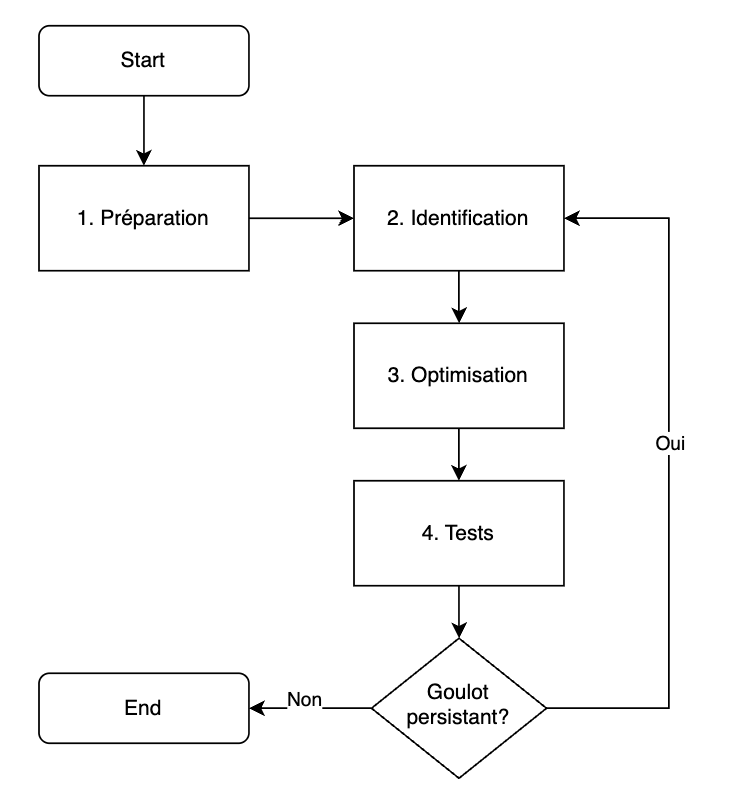
\includegraphics[width=0.5\textwidth]{img/mesure-analyse-opti.png}
    \caption{Cycle itératif mesure--analyse--optimisation.}
    \label{fig:opti-cycle}
\end{figure}

% - - - - - - - - - - -
\section{Environnement expérimental et outils de mesure}
\label{sec:env}
% - - - - - - - - - - -

\paragraph{Configuration matérielle et logicielle.}
Les expériences ont été réalisées sur une machine équipée d'un processeur AMD
Ryzen 5 9600X (6 cœurs, 12 threads, 65W TDP), disposant de 32~Go de mémoire
vive DDR5 cadencée à 6000~MHz et d'un stockage SSD NVMe. Ce choix matériel
vise à minimiser l'impact des I/O disque et de la latence mémoire sur les
mesures, de sorte que les goulots observés reflètent le comportement applicatif
plutôt que les limitations de l'infrastructure.

Le système d'exploitation est Linux (architecture x86\_64). L'environnement
d'exécution est Java 8 (JDK 1.8), qui correspond à la version cible de
MetaDONE déployée dans Eclipse Oxygen (4.7.0). Ce choix contraint certaines
options de collecteur GC disponibles dans les versions ultérieures du JDK
(ZGC et Shenandoah n'étant disponibles qu'à partir de Java 11 et 12
respectivement), mais garantit la fidélité des résultats à l'environnement
de production réel de l'outil.

\paragraph{Reproductibilité des mesures.}
Chaque scénario a été exécuté 10 fois et les résultats présentés correspondent aux valeurs médianes des 10 mesures. La médiane est préférée à la moyenne car elle est plus robuste aux valeurs aberrantes liées aux pauses du \textit{Garbage Collector} ou aux interruptions du système d'exploitation~\cite{georges2007statistically}~: avec 10 répétitions, elle absorbe jusqu'à 4 valeurs aberrantes sans biais. Pour chaque scénario, le \textbf{coefficient de variation} (CV~$= \sigma / \mu$) a également été calculé afin de vérifier la stabilité des mesures~: un CV faible (typiquement inférieur à 5\,\%) confirme que 10 répétitions sont suffisantes pour obtenir une médiane stable. Aucune phase de warmup de la JVM n'a en revanche été instaurée, faute de temps~; cette limite est discutée au chapitre~\ref{chap:discussion}, où l'on s'assure que les ordres de grandeur des gains observés en sont peu affectés.

\paragraph{Outils de profilage.}
Deux outils complémentaires ont été retenus, dont le choix est justifié dans
le tableau~\ref{tab:profilers}.

\begin{table}[h]
\centering
\caption{Comparaison des principaux outils de profilage Java}
\label{tab:profilers}
\small
\begin{tabular}{lllll}
\hline
\textbf{Outil} & \textbf{Méthode} & \textbf{Surcoût} &
\textbf{Domaine} & \textbf{Visualisation} \\
\hline
JVisualVM    & Sampling/instrum. & Moyen    & CPU, heap       & GUI intégrée \\
JFR + JMC    & Sampling faible   & Très faible & CPU, GC, I/O, locks & Flight Recorder \\
async-profiler & Perf events     & Quasi nul & CPU (wall/alloc) & Flamegraph SVG \\
JProfiler    & Instrumentation   & Élevé    & CPU, mémoire, JDBC & GUI riche \\
YourKit      & Sampling/instrum. & Moyen    & CPU, mémoire    & GUI riche \\
\hline
\end{tabular}
\end{table}

Parmi les cinq outils du tableau~\ref{tab:profilers}, seuls \textbf{JFR} et \textbf{async-profiler} ont été retenus. JVisualVM, JProfiler et YourKit ont été écartés en raison d'un surcoût d'instrumentation jugé incompatible avec des mesures représentatives à grande échelle.

\textbf{Java Flight Recorder (JFR)} est utilisé pour les mesures de
durée globale et l'analyse des événements GC, des locks et des accès I/O
sur l'ensemble d'un scénario. Son surcoût inférieur à 1\,\% en fait
l'outil de référence pour les mesures de longue durée sans biais
d'observation~\cite{jfr2021oracle}.

\textbf{async-profiler}~\cite{asyncprofiler} est utilisé pour localiser précisément les
méthodes chaudes (\textit{hotspots}) via des flamegraphs. Il s'appuie sur
les compteurs de performance matériels du CPU via \texttt{perf\_events}
plutôt que sur l'instrumentation JVM, ce qui élimine le biais du
\textit{safepoint sampling} qui affecte les profileurs JVM classiques~\cite{mytkowicz2010evaluating}. Les deux outils sont complémentaires~: JFR mesure \textit{quoi} et \textit{combien}, async-profiler localise \textit{où}.

\section[Scénarios représentatifs]{Scénarios représentatifs des usages de MetaDONE}
\label{sec:scenarios}

La sélection des scénarios suit trois critères~: la \textbf{fréquence} (les
opérations exécutées à chaque session de travail), la \textbf{criticité}
(les opérations dont la latence est directement perçue par l'utilisateur)
et la \textbf{scalabilité} (les opérations dont le coût croît avec la
taille du projet et qui révèlent d'éventuelles dégradations non-linéaires).
Les deux premiers critères sont cohérents avec la recommandation générale
de concentrer les efforts sur les chemins d'exécution à fort
impact~\cite{oaks2014java}~; le troisième complète cette démarche en
exposant les hypothèses architecturales à l'épreuve du volume.

Quatre scénarios ont finalement été retenus, couvrant des parties significatives du cycle de vie d'une session MetaDONE~\footnote{Un cinquième scénario, dédié à la modification et au rechargement itératif d'un script GraSyLa, avait initialement été planifié sous le numéro S3, mais a été écarté en cours de mémoire au profit d'une analyse plus approfondie de la boucle de visualisation (S4). La numérotation des scénarios suivants a été conservée pour rester cohérente avec les comptes-rendus intermédiaires.}~:

\begin{description}
    \item[Scénario~1~: Phase d'initialisation.] Au démarrage de MetaDONE, le dépôt est ouvert et les items séminaux de MetaL$_1$ ainsi que le métamétamodèle MetaL$_2$ sont chargés depuis la base de données. Cette phase est exécutée à chaque lancement et constitue le premier point de friction pour l'utilisateur. Elle implique la résolution des cycles de la relation \texttt{instanceOf} décrits à la section~\ref{sec:graphes-cycliques}, et constituera donc l'occasion de tester l'hypothèse formulée en section~\ref{sec:persistance-openjpa} selon laquelle ce chargement souffrirait du problème du N+1 et des limites du lazy loading.

    \item[Scénario~2~: Chargement d'un script GraSyLa.] L'ouverture d'un
    projet existant nécessite le chargement du script GraSyLa associé à son
    métamodèle, puis la construction de l'arbre d'expressions correspondant
    en mémoire. Ce scénario implique des traversées répétées du graphe
    méta-circulaire et est représentatif des sessions de modélisation
    quotidiennes.

    \item[Scénario~4~: Visualisation d'un (méta)modèle.] Le rendu graphique d'un modèle par GraSyLa implique l'évaluation de l'ensemble des équations du script pour chaque objet du modèle. Sur des modèles de taille significative, ce scénario met en évidence les coûts de traversée de graphe et d'évaluation des expressions.

    \item[Scénario~5~: Création et persistance d'un grand modèle (réseau de Petri).] Pour évaluer le comportement de MetaDONE à l'échelle, ce scénario construit programmatiquement un réseau de Petri de taille croissante, le visualise, puis le sauvegarde dans le dépôt. Il permet d'évaluer la scalabilité de la persistance JPA sur des volumes importants d'éléments de même type et de vérifier l'absence de dégradation non-linéaire des performances. Ce scénario relève moins de l'usage quotidien que des deux premiers et illustre le critère de scalabilité introduit ci-dessus.
\end{description}

Ces scénarios sont traités dans les sections suivantes selon le cycle itératif décrit à la section~\ref{sec:cycle}. Chaque section commence par une description de la baseline mesurée, puis alterne phases d'identification et d'optimisation jusqu'à convergence vers un résultat satisfaisant ou jusqu'à identification d'une limite structurelle de l'architecture actuelle.